\documentclass[../main/main.tex]{subfiles}

\newdate{date}{30}{11}{2020}

% \begin{figure}[h!]
% \centering
% \includegraphics[page=6,width=0.8\textwidth]{../lessons/pdf_file/21_lecture.pdf}
% \end{figure}

%\displaydate{date}. Compiled:  \today. Alice.

\begin{document}

\pagestyle{plain}

\section{Lecture 21}


\subsubsection*{Slide 1}

\begin{minipage}[]{0.5\linewidth}
\centering
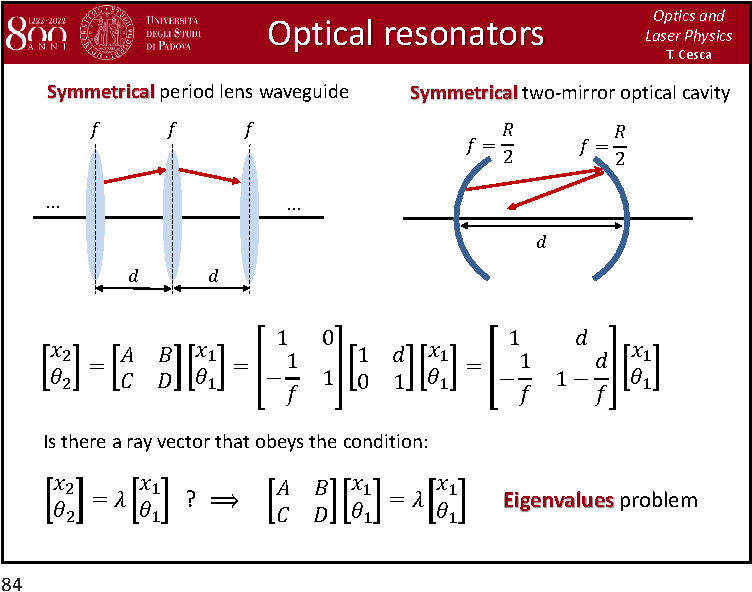
\includegraphics[page=1,width=1\textwidth]{../lessons/pdf_file/21_lecture.pdf}
\end{minipage}
\hspace{0.3cm}\vspace{0.3cm}
\begin{minipage}[c]{0.47\linewidth}

Let us apply ABCD method to optical resonators. Firstly, we describe \textbf{symmetrical} optical resonators. We can have a sequence of thin lenses separated by distance \( d \).
Or, we can think about the optical resonator as formed by two spherical mirrors.

Let us stress the sign convention. When we consider mirror, differently from before, we will consider that a \textbf{concave} mirror has a \textbf{positive} radius of curvature: so the focal length is half the radius of curvature. In the previous lessons, the concave mirror had a negative radius of curvature.

Moreover, when we will discuss optical resonator, we consider as we are inside the cavity and we turn our head once from one side and one from the other and we see the two mirrors has both concave! This is different if you think to be outside the cavity.

The signs will be according to this new convention!

\end{minipage}

The basic unit for this description is simply a propagation for a distance \( d \) and then the interaction for an optical element with focal length \( f \). This is the same for a period lens waveguid or a for two-mirror optical cavity.

There exist a ray vector which is an eigenstate of this system just after one pass? We have an \textbf{eigenvalue problem}.

\subsubsection*{Slide 2}

\begin{minipage}[]{0.5\linewidth}
\centering
\includegraphics[page=2,width=1\textwidth]{../lessons/pdf_file/21_lecture.pdf}
\end{minipage}
\hspace{0.3cm}\vspace{0.3cm}
\begin{minipage}[c]{0.47\linewidth}

We have a \textbf{stable} and an \textbf{unstable} solutions (as we will see).

\end{minipage}

\subsubsection*{Slide 3}

\begin{minipage}[]{0.5\linewidth}
\centering
\includegraphics[page=3,width=1\textwidth]{../lessons/pdf_file/21_lecture.pdf}
\end{minipage}
\hspace{0.3cm}\vspace{0.3cm}
\begin{minipage}[c]{0.47\linewidth}

Let us consider when the resonator is stable (\( \abs{g} \le 1  \)). It means that the two solution are imaginary. For a large number of passes inside the resonator, you will still have the same eigenvalue. It means that the modulus is still 1: it will keep the same coordinates.

For \( \abs{g} \ge 1  \), the eigenvalues are real numbers and the trajectory will diverge at each pass. The ray will not stay inside the cavity but will escape from it after a given number of passes.

\end{minipage}

\newpage

\subsubsection*{Slide 4}

\begin{minipage}[]{0.5\linewidth}
\centering
\includegraphics[page=4,width=1\textwidth]{../lessons/pdf_file/21_lecture.pdf}
\end{minipage}
\hspace{0.3cm}\vspace{0.3cm}
\begin{minipage}[c]{0.47\linewidth}

The \textbf{stability condition} can be rewritten in terms of the distance \( d \) that has to be smaller than \( 4 f \). We can rewrite it also in terms of the radius of curvature.

\end{minipage}

\subsubsection*{Slide 5}

\begin{minipage}[]{0.5\linewidth}
\centering
\includegraphics[page=5,width=1\textwidth]{../lessons/pdf_file/21_lecture.pdf}
\end{minipage}
\hspace{0.3cm}\vspace{0.3cm}
\begin{minipage}[c]{0.47\linewidth}

Let us consider the most complex of \textbf{asymetrical resonators}. For instance we have two different radius of curvature for the two mirrors (two different focal lengths). The sign convention is exactly the same.
For a sequence of thin lenses we have different focal lengths.

Now, the basic unit is slightly different from before. The unit that is repeated more times is given by the propagation from the first focal length, the propagation on free space, the propagation from the second focal length and the propagation in free space. Then, we start again.

\end{minipage}

\subsubsection*{Slide 6}

\begin{minipage}[]{0.5\linewidth}
\centering
\includegraphics[page=6,width=1\textwidth]{../lessons/pdf_file/21_lecture.pdf}
\end{minipage}
\hspace{0.3cm}\vspace{0.3cm}
\begin{minipage}[c]{0.47\linewidth}

Let us solve again the eigenvalue problem. We end up again in a second order equation.

Now, the stability condition is \( \abs{\alpha }\le 1  \) in order to have compelx eigenvalues.

\end{minipage}

\newpage

\subsubsection*{Slide 7}

\begin{minipage}[]{0.5\linewidth}
\centering
\includegraphics[page=7,width=1\textwidth]{../lessons/pdf_file/21_lecture.pdf}
\end{minipage}
\hspace{0.3cm}\vspace{0.3cm}
\begin{minipage}[c]{0.47\linewidth}

We can introduce two factors, the condition of stability can be given in terms of their product.

The symmetric case is just a particular case of the asymmetric condition.

\end{minipage}

\subsubsection*{Slide 8}

\begin{minipage}[]{0.5\linewidth}
\centering
\includegraphics[page=8,width=1\textwidth]{../lessons/pdf_file/21_lecture.pdf}
\end{minipage}
\hspace{0.3cm}\vspace{0.3cm}
\begin{minipage}[c]{0.47\linewidth}

We can represent the stability condition in terms of a plot.

These stability condition corresponds to the dashed region on the plot.

The axis are the point given by \( g_1 g_2 = 0 \). Instead, for \( g_1 g_2 = 1 \) we have the black lines.

All the points which belong to the axis or to the hyperboles represent the optical cavity with \textbf{marginal stability}.

All the points inside the dashed regions are in the \textbf{stability} condition.

All the points outside they represent and \textbf{unstable} resonator.

\end{minipage}

\subsubsection*{Slide 9}

\begin{minipage}[]{0.5\linewidth}
\centering
\includegraphics[page=9,width=1\textwidth]{../lessons/pdf_file/21_lecture.pdf}
\end{minipage}
\hspace{0.3cm}\vspace{0.3cm}
\begin{minipage}[c]{0.47\linewidth}

The point C represent the \textbf{Fabry-Perot cavity}. Indeed, we have two plane mirrors (\( R_1 = R_2 = \infty  \)).

The point B represent a \textbf{confocal resonator}.

The point A represent a \textbf{concentric resonator}.

These are symmetric configuration.
Moreover, all the configurations along the black line (bisector) represent symmetric configuration and stable.

Physically, a condition of marginal stability means that it is easy to get out from the stability region. It means that a slightly disallignment can get out from the stability condition.

If you are in any of the point inside the dashed region, you will stay inside the stability region if you move slightly from these. So, they are more stable from this point of view.

\end{minipage}

\subsubsection*{Slide 10}

\begin{minipage}[]{0.5\linewidth}
\centering
\includegraphics[page=10,width=1\textwidth]{../lessons/pdf_file/21_lecture.pdf}
\end{minipage}
\hspace{0.3cm}\vspace{0.3cm}
\begin{minipage}[c]{0.47\linewidth}

The dashed hyperboles represent possible confocal resonator. Apart from the configuration B, all the others will be unstable. One example of them is in D. We write \( -d \) because for solving the problem from this point of view, the convention we are adopting is looking at the mirror from inside the cavity.

\end{minipage}

\subsubsection*{Slide 11}

\begin{minipage}[]{0.5\linewidth}
\centering
\includegraphics[page=11,width=1\textwidth]{../lessons/pdf_file/21_lecture.pdf}
\end{minipage}
\hspace{0.3cm}\vspace{0.3cm}
\begin{minipage}[c]{0.47\linewidth}

This is another example of a confocal configuration but in a negative branch. We have two concave mirrors.

\end{minipage}

\subsubsection*{Slide 12}

\begin{minipage}[]{0.5\linewidth}
\centering
\includegraphics[page=12,width=1\textwidth]{../lessons/pdf_file/21_lecture.pdf}
\end{minipage}
\hspace{0.3cm}\vspace{0.3cm}
\begin{minipage}[c]{0.47\linewidth}

Let us try to solve na exercise. What is the maximum distance at which we can place the two mirrors to make the resonator stable? 

\end{minipage}


\end{document}
